\documentclass[12pt,a4paper]{report}
\usepackage[utf8]{inputenc}
\usepackage{vietnam}
\usepackage{geometry}
\usepackage{amsmath}
%\usepackage{asmfonts}
\usepackage{float}
\usepackage{amssymb} 
\usepackage{graphicx} % thư viện hiển thị hình ảnh
\usepackage[hidelinks, unicode]{hyperref} % thư viện link tới chương
\usepackage{caption} % thư viện đặt caption
\usepackage[table]{xcolor} % thư viện hiển thị màu cho bảng
\usepackage{titletoc}
\usepackage{etoc}
%\usepackage{indentfirst}
\usepackage{mathptmx}
\usepackage{sectsty}
\usepackage{tikz}
\usepackage{booktabs}

\makeatletter
\titlecontents{chapter}[3cm] % <-- seems to set some specific left margin
{\color{black}\bfseries\addvspace{3mm}}
{\makebox[0cm][r]{\MakeUppercase\@chapapp\hspace{.5em}\thecontentslabel\hspace{0.75cm}}}
{} %     ^^^ pretendously zero width box puts its contents in the left margin
{\hfill\makebox[-2cm]{\thecontentspage}}  % 3cm = twice 1.5cm
\chapternumberfont{\Large}
\chaptertitlefont{\Large}



\renewcommand{\baselinestretch}{1.5}
\newcommand{\subsubsubsection}[1]{\paragraph{#1}\mbox{}\\}

\setlength\parindent{0pt}
\setcounter{secnumdepth}{4}
\setcounter{tocdepth}{4}
\geometry{letterpaper}
\title{\textbf{BÁO CÁO THỰC TẬP}}
\author{Bui Trong Nghia}

\begin{document}
\pagenumbering{roman}
\thispagestyle{empty}
\clearpage


\pdfbookmark{\contentsname}{content}
\maketitle
\newpage

\begin{center}
	\centering
    \textbf{LỜI CẢM ƠN}
\end{center}
Thành công của một cá nhân luôn luôn gắn liền với sự giúp đỡ, hỗ trợ dù ít hay nhiều, dù trực tiếp hay gián tiếp của những người khác. Trong suốt quãng đường từ khi em mới bắt đầu học tập tại giảng đường trường Đại Học Dầu Khí Việt Nam cho đến nay, em đã nhận được rất nhiều sự quan tâm giúp đỡ của các quý Thầy Cô, gia đình và bạn bè.\\
Với lòng biết ơn sâu sắc nhất, em xin gửi đến quý Thầy Cô ở khoa Dầu Khí – trường Đại Học Dầu Khí Việt Nam đã cùng với tri thức và tâm huyết của mình để truyền đạt vốn kiến thức quý báu cho chúng em trong suốt thời gian học tập tại trường. Và đặc biệt, trong học kì này, khoa đã tạo điều kiện cho em thực tập tại phòng Công nghệ mỏ, Công ty Dầu khí Việt - Nhật.\\
Em cũng xin chân thành cám ơn ban lãnh đạo và các Anh, Chị trong JVPC, đặc biệt là anh Hà Anh Dũng và anh Nguyễn Phúc Huy đã giúp đỡ nhiệt tình, tạo điều kiện thuận lợi nhất để em có thể hoàn thành tốt thời gian thực tập này. Vì là lần đầu tiên em được thực tập tại quý công ty nên không thể tránh được những thiếu sót trong quá trình học tập, em rất mong nhận được sự bỏ qua và những ý kiến đóng góp của Anh, Chị giúp em hoàn thiện hơn.\\
Bài báo cáo thu hoạch được thực hiện trong khoảng thời gian hai tuần. Bước đầu tìm hiểu về lĩnh vực công nghệ mỏ trong thực tế. Bởi vì kiến thức còn hạn chế và còn nhiều bỡ ngỡ, do vậy, không tránh khỏi thiếu sót là điều chắc chắn. Em rất mong nhận được những ý kiến quý báu của quý Thầy Cô và các bạn học cùng lớp để kiến thức của em trong lĩnh vực này được ngày một hoàn thiện hơn.\\
Sau cùng, em xin kính chúc quý Thầy Cô khoa Dầu khí, trường Đại Học Dầu Khí Việt Nam và toàn thể Anh, Chị phòng Công nghệ mỏ, Công ty Dầu khí Việt - Nhật dồi dào sức khỏe và đạt được nhiều thành công trong công việc.\\
Trân trọng.

\newpage
\tableofcontents
\listoffigures
%\listoftables
\clearpage
\pagenumbering{arabic}
\newpage

\chapter{KHÁI QUÁT VỀ ĐƠN VỊ THỰC TẬP}
\section{Tổng quan, lịch sử hình thành, cơ cấu tổ chức và chức năng nhiệm vụ của Công ty Liên doanh JVPC}
\subsection{Tổng quan}
Tên đầy đủ: Công ty Liên doanh Dầu khí Việt - Nhật.\\
Tên tiếng anh: Japan Vietnam Petroleum Company.\\
Tên gọi tắt: JVPC\\
Trụ sở văn phòng: Tầng 7, tòa nhà PetroVietnam, số 8 đường Hoàng Diệu, tp. Vũng Tàu, tỉnh Bà Rịa - Vũng Tàu.

\subsection{Lịch sử hình thành}
Công ty TNHH Dầu khí Việt Nhật (JVPC) được thành lập và hoạt động tại Việt Nam từ năm 1992. Sau những năm đầu thực hiện xây dựng cơ sở vật chất phục vụ việc hoạt động khai thác dầu thô, đến năm 1998 JVPC đã khai thác thùng dầu đầu tiên, năm 2005 khai thác thùng dầu thứ 100 triệu, năm 2006 bắt đầu hoạt động thu gom khí đồng hành, đến cuối tháng 8-2007 đạt sản lượng khai thác 138 triệu thùng dầu và 2,7 tỷ m3 khí đồng hành.\\
Sau hơn 20 năm hoạt động tại Việt Nam, JVPC đã khẳng định được vị thế và uy tín trong ngành dầu khí Việt Nam. Trong quá trình hoạt động, JVPC luôn bảo đảm công tác an toàn và bảo vệ môi trường, thực hiện tốt nghĩa vụ nộp thuế. Bên cạnh hoạt động sản xuất, JVPC còn tích cực tham gia các hoạt động xã hội từ thiện trên địa bàn tỉnh Bà Rịa-Vũng Tàu.
\subsection{Lịch sử phát triển Lô 15-2}
	\begin{itemize}
    	\item[1992] Kí kết hợp đồng quản lý khai thác (PSC) ở Lô 15-2 với PetroVietnam
        \item[1994] Khoan giếng thăm dò đầu tiên
        \item[1996] Tuyên bố khả năng thương mại của mỏ Rạng Đông
        \item[1997] PVEP tham gia vào dự án
        \item[1998] Dòng dầu đầu tiên tại đầu giếng WHP-N1
        \item[2000] ConocoPhillips tham gia vào dự án
        \item[2001] Bắt đầu khai thác khí đồng hành
        \item[2002] Dòng dầu đầu tiên tại các đầu giếng WHP-E1, WHP-S1. Thùng dầu thứ 50 triệu vào ngày 3 tháng 9.
        \item[2003] Ứng dụng các phương pháp khai thác bơm ép khí, nước.
        \item[2005] Dòng dầu đầu tiên tại WHP-C1. Thùng dầu thứ 100 triệu vào ngày 12 tháng 6.
        \item[2006] Áp dụng công nghệ khai thác khí sạch
        \item[2007] Tuyên bố khả năng thương mại của mỏ Phương Đông
        \item[2008] Dòng dầu đầu tiên tại mỏ Phương Đông. Thùng dầu thứ 150 triệu ngày 21 tháng 7.
        \item[2012] Hoàn thành đầu giếng khai thác WHP-E1A
        \item[2014] Thùng dầu thứ 200 triệu vào ngày 8 tháng 7. Áp dụng công nghệ khai thác dầu tăng cường cho mỏ Rạng Đông
        \item[2017] Kỉ niệm 25 năm ngày bắt đầu các hoạt động tìm kiếm, thăm dò và khai thác tại Lô 15-2 trên vùng biển Việt Nam.
    \end{itemize}
\subsection{Cơ cấu tổ chức}
Bộ máy Công ty Liên doanh Dầu khí Việt - Nhật bao gồm:
	\begin{enumerate}
    	\item General Director - Mr. Yuri Kurata
        \item Deputy General Director - Mr. Nguyen Hoai Anh
        \item General Affairs Department - Ms. Nguyen Thi Thu
        \item Contract \& Business Development Department - Mr. Do Ngoc Thanh
        \item HSE \& Offtake Operations Department - Mr. Nguyen Hoai Anh
        \item Technical Department - Mr. Nguyen Chu Chuyen
        \item Well Operation Department - Mr. Ha The Giang
        \item Production Operation Department - Mr. Tran Van Hien
    \end{enumerate}
\subsection{Chức năng, nhiệm vụ}
Điều hành quản lý các hoạt động khoan, khai thác và phát triển của các giếng khoan ở hai mỏ Rạng Đông và Phương Đông thuộc Lô 15-2 bể Cửu Long Thềm lục địa Việt Nam.
\section{Phòng Công nghệ mỏ}
%\subsection{Cơ cấu tổ chức}
	\begin{enumerate}
    	\item Group Manager - Mr. Takahiro Murakami
        \item Senior Reservoir Engineer - Mr. Alexandre Charles Henri Nappez
        \item Senior Reservoir Engineer - Mr. Vu Thanh
        \item Reservoir Engineer - Mr. Dao Cong Thien
        \item Reservoir Engineer - Mr. Shin Kamioka
        \item Reservoir Engineer - Mr. Ha Minh Dung
        \item Reservoir Engineer - Mr. Nguyen Phuc Huy
        \item Reservoir Engineer - Ms. Aiko Imai
        \item Reservoir Engineer - Mr. Kazuaki Mikami
        \item Administrator - Ms. Le Thi Lan Huong
    \end{enumerate}

\chapter{KẾT QUẢ THỰC TẬP}
\section{Nội dung công việc được giao}
\subsection{Nội dung và mục tiêu}
\textbf{Nội dung:}
	\begin{itemize}
    	\item[-] Xây dựng mộ hình dự báo khai thác.
	\end{itemize}
\textbf{Mục tiêu}
	\begin{itemize}
    	\item[-] Tối ưu hóa lưu lượng khai thác dầu bằng mô hình mới xây dựng dựa trên lưu lượng gas lift.
    \end{itemize}
\subsection{Phương pháp tiến hành, tiến độ và kết quả}
\textbf{Phương pháp tiến hành:} Kết hợp kiến thức phân tích dự báo khai thác, tối ưu khai thác với trí tuệ nhân tạo .\\
\textbf{Kết quả:} Xây dựng được mô hình dựa trên code Python.
\subsection{Tự nhận xét về mức độ hoàn thành công việc được giao}
Hoàn thành cơ bản công việc được giao.
\section{Những kiến thức, kĩ năng và kinh nghiệm thu được}
	\begin{itemize}
    	\item[-] Phân tích tối ưu khai thác.
    \end{itemize}
\chapter{NỘI DUNG KẾT QUẢ THỰC TẬP}
\section{Giếng X1}
Giếng X1 được lựa chọn cho quá trình thực hiện xây dựng mô hình dựa trên cơ sở:
    \begin{itemize}
        \item Dữ liệu giếng thuộc loại dữ liệu cấu trúc,
        \item Dữ liệu được ghi lại theo thời gian,
        \item Thuộc mỏ Rạng Đông.
    \end{itemize}
\section{Phương pháp}
Xây dựng mô hình với mạng neuron nhân tạo truyền thẳng (Multi-layer Perceptron, MLP) với các đặc tính:
    \begin{itemize}
        \item Dễ dàng cấu trúc và sử dụng,
        \item Hiệu suất cao,
        \item Phù hợp cho dữ liệu có cấu trúc,
        \item Phù hợp với dữ liệu theo thời gian.
    \end{itemize}
Đánh giá tính chính xác của mô hình dựa trên các chỉ số  bình phương tối thiểu và $R^2$.
\def\layersep{2.5cm}
\begin{tikzpicture}[shorten >=1pt,->,draw=black!50, node distance=\layersep]
    \tikzstyle{every pin edge}=[<-,shorten <=1pt]
    \tikzstyle{neuron}=[circle,fill=black!25,minimum size=17pt,inner sep=0pt]
    \tikzstyle{input neuron}=[neuron, fill=green!50];
    \tikzstyle{output neuron}=[neuron, fill=red!50];
    \tikzstyle{hidden neuron}=[neuron, fill=blue!50];
    \tikzstyle{annot} = [text width=4em, text centered]

    % Draw the input layer nodes
    \foreach \name / \y in {1,...,4}
    % This is the same as writing \foreach \name / \y in {1/1,2/2,3/3,4/4}
        \node[input neuron, pin=left:Input \#\y] (I-\name) at (0,-\y) {};

    % Draw the hidden layer nodes
    \foreach \name / \y in {1,...,5}
        \path[yshift=0.5cm]
            node[hidden neuron] (H-\name) at (\layersep,-\y cm) {};

    % Draw the output layer node
    \node[output neuron,pin={[pin edge={->}]right:Output}, right of=H-3] (O) {};

    % Connect every node in the input layer with every node in the
    % hidden layer.
    \foreach \source in {1,...,4}
        \foreach \dest in {1,...,5}
            \path (I-\source) edge (H-\dest);

    % Connect every node in the hidden layer with the output layer
    \foreach \source in {1,...,5}
        \path (H-\source) edge (O);

    % Annotate the layers
    \node[annot,above of=H-1, node distance=1cm] (hl) {Hidden layer};
    \node[annot,left of=hl] {Input layer};
    \node[annot,right of=hl] {Output layer};
\end{tikzpicture}
\newline
Hình trên mô tả một mạng MLP cơ bản với 1 lớp đầu vào với 4 nút, 1 lớp ẩn với 5 nút, 1 lớp đầu ra với 1 nút.
\section{Chuẩn bị dữ liệu}
    \begin{table}[h]
    \centering
    \caption{Giếng X1}
    \begin{tabular}{@{}ccccccc@{}}
    \toprule
    \textbf{\begin{tabular}[c]{@{}c@{}}WHFP\\ psi\end{tabular}} & \textbf{\begin{tabular}[c]{@{}c@{}}WHFT\\ deg C\end{tabular}} & \textbf{\begin{tabular}[c]{@{}c@{}}WCT\\ \%bbl/bbl\end{tabular}} & \textbf{\begin{tabular}[c]{@{}c@{}}GOR\\ cf/bbl\end{tabular}} & \textbf{\begin{tabular}[c]{@{}c@{}}BHP\\ psi\end{tabular}} & \textbf{\begin{tabular}[c]{@{}c@{}}Qgl\\ Mcf/d\end{tabular}} & \textbf{\begin{tabular}[c]{@{}c@{}}Qo\\ SBT/D\end{tabular}} \\ \midrule
    902.83                                                      & 29.26                                                         & NaN                                                              & 0                                                             & 4786.92                                                    & 0                                                            & 0                                                           \\
    1118.07                                                     & 30.02                                                         & NaN                                                              & 0                                                             & 3638.66                                                    & 0                                                            & 0                                                           \\
    ...                                                         & ...                                                           & ...                                                              & ...                                                           & ...                                                        & ...                                                          & ...                                                         \\
    204.98                                                      & 62.2                                                          & 91.05                                                            & 333                                                           & 2715.62                                                    & 1104                                                         & 153.27                                                      \\
    202.45                                                      & 62.63                                                         & 91.14                                                            & 329                                                           & 2702.48                                                    & 1096                                                         & 152                                                         \\ \bottomrule
    \end{tabular}
    \end{table}
\newpage
Dữ liệu giếng X1 bắt đầu được đo đạt từ ngày 6/2/2014 đến 2/6/2019, với 1720 điểm dữ liệu, 42 điểm mất mát tại đặc tính water cut.
    \begin{figure}[h]
        \centering
        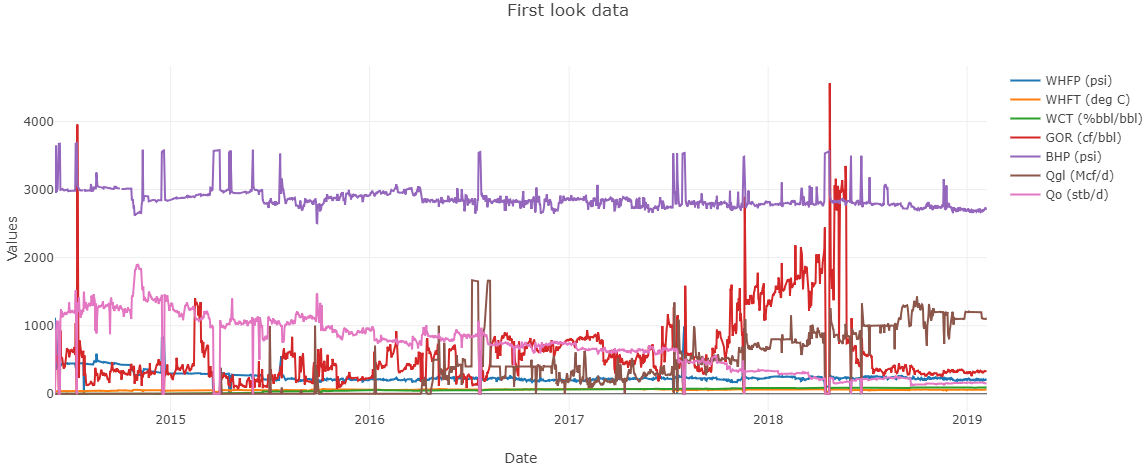
\includegraphics[scale=.55]{fig/first_look.PNG}
        \caption{Dữ liệu ban đầu của giếng X}
        \label{fig:first_look}
    \end{figure}
\newline
\subsection{Làm sạch giữ liệu}
Dựa trên sự phụ thuộc của dữ liệu đầu ra đôi với dữ liệu đầu vào và các tiêu chí tối ưu hóa các đặc tính được lựa chọn đưa vào mô hình:
    \begin{itemize}
        \item Water cut
        \item Tỉ lệ khí - dầu
        \item Lưu lượng gas lift.
    \end{itemize}
Dữ liệu đầu ra sẽ là lưu lượng dầu theo thời gian.\\
Dữ liệu sẽ được làm sạch để có thể đem lại kết quả tốt hơn. Các phương pháp làm sạch như sau:
    \begin{itemize}
        \item Xử lí các điểm ngoại lai,
        \item Loại bỏ các điểm bằng 0,
        \item Xử lí các điểm dữ liệu mất mát.
    \end{itemize}
Thuộc tính water cut sẽ được giữ nguyên, không cần xử lý do không chứa các điểm ngoại lai hay nhiễu.
    \begin{figure}[h]
        \centering
        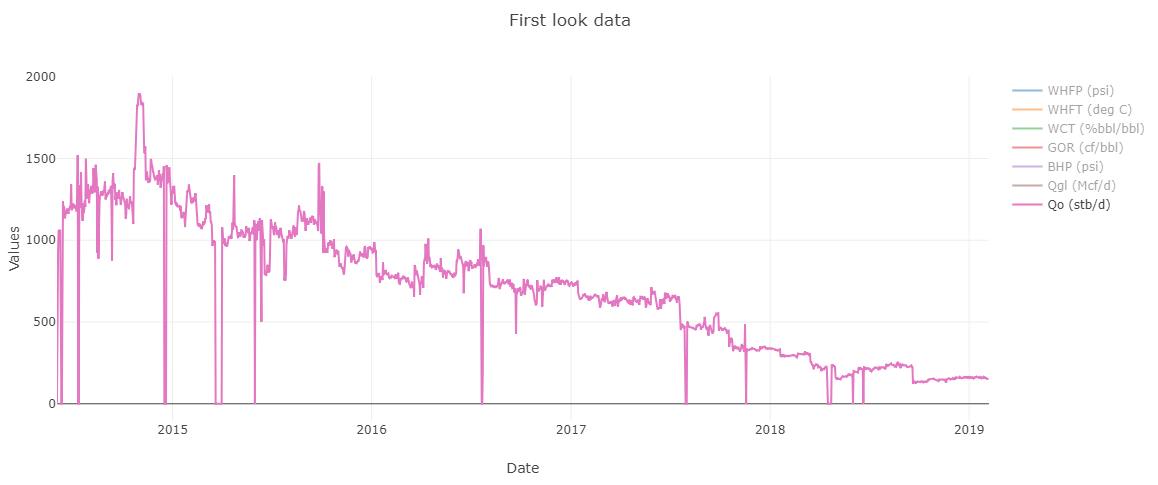
\includegraphics[scale=0.55]{fig/q_oil_before.PNG}
        \caption{Lưu lượng dầu chưa được xử lý}
        \label{fig:q_oil_before}
    \end{figure}
    \begin{figure}[h]
        \centering
        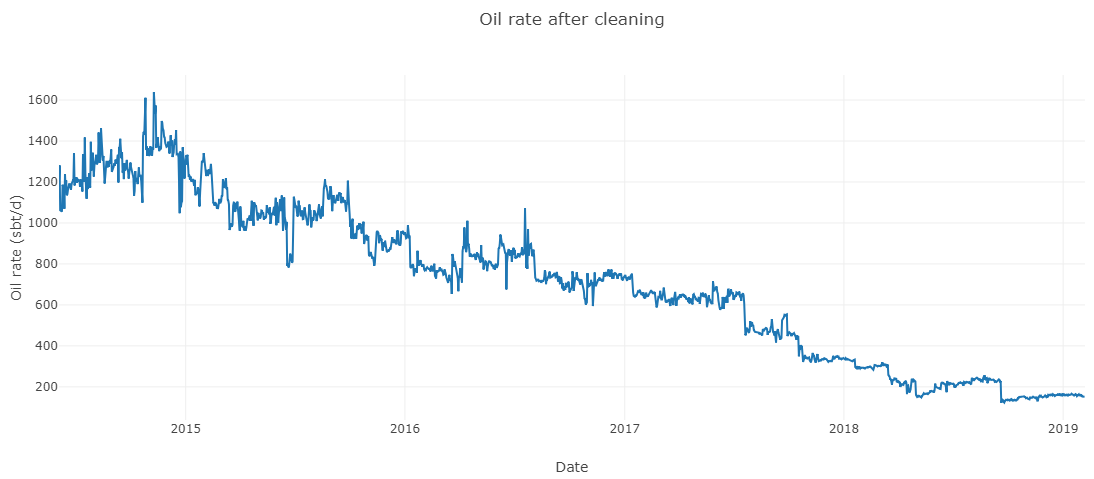
\includegraphics[scale=.55]{fig/q_oil_after.PNG}
        \caption{Lưu lượng dầu đã được xử lý}
        \label{fig:q_oil_after}
    \end{figure}
    \begin{figure}[h]
        \centering
        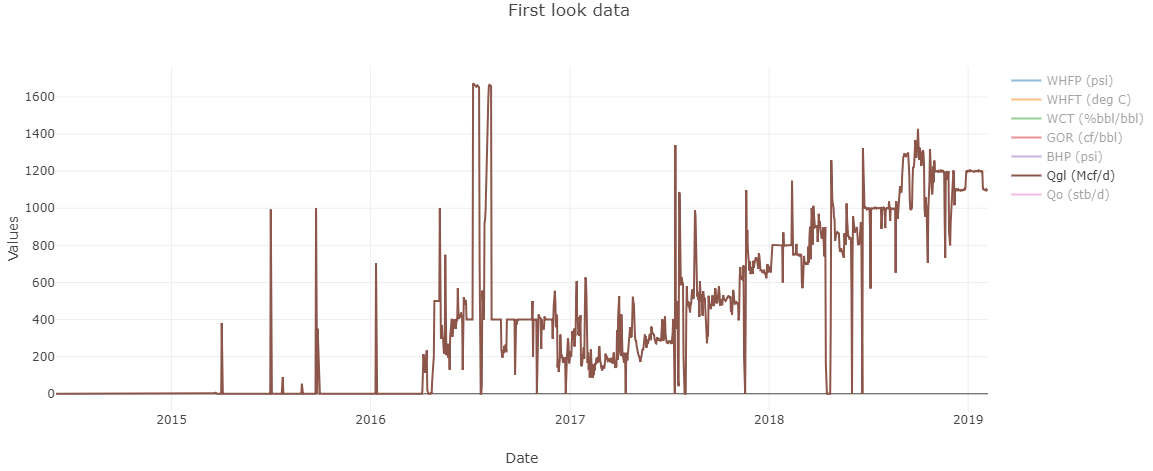
\includegraphics[scale=0.55]{fig/gl_before.PNG}
        \caption{Lưu lượng gaslift chưa được xử lý}
        \label{fig:gl_before}
    \end{figure}
    \begin{figure}[h]
        \centering
        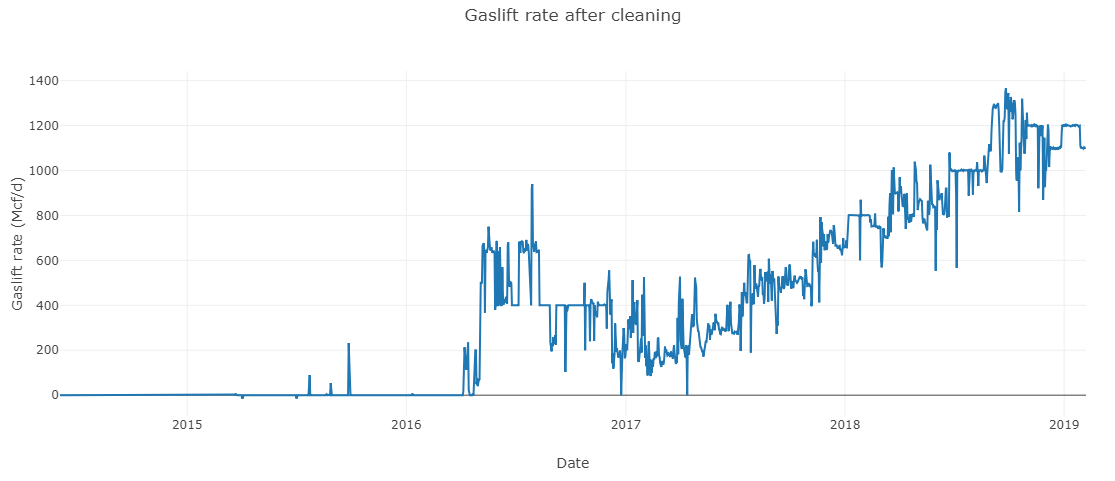
\includegraphics[scale=0.55]{fig/gl_after.PNG}
        \caption{Lưu lượng gaslift đã được xử lý}
        \label{fig:gl_after}
    \end{figure}
    \begin{figure}[h]
        \centering
        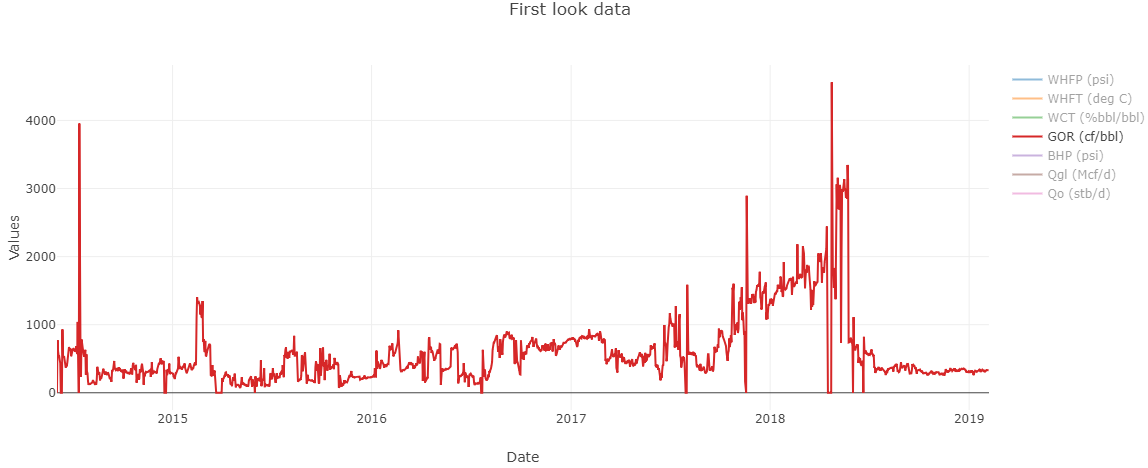
\includegraphics[scale=0.55]{fig/gor_before.PNG}
        \caption{Tỉ số khí dầu chưa được xử lý}
        \label{fig:gor_before}
    \end{figure}
    \begin{figure}[h]
        \centering
        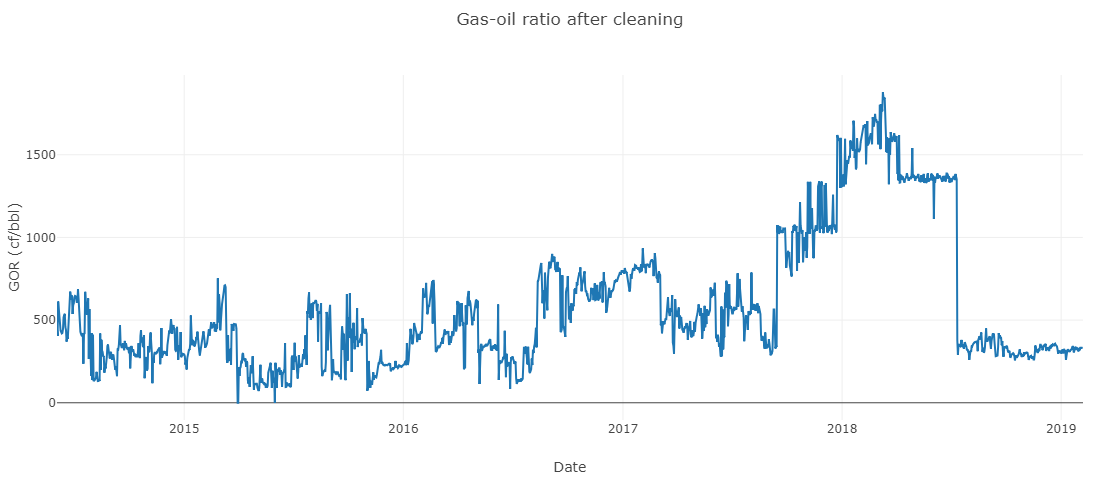
\includegraphics[scale=0.55]{fig/gor_after.PNG}
        \caption{Tỉ số khí dầu đã được xử l}
        \label{fig:gor_after}
    \end{figure}
    \begin{figure}[h]
        \centering
        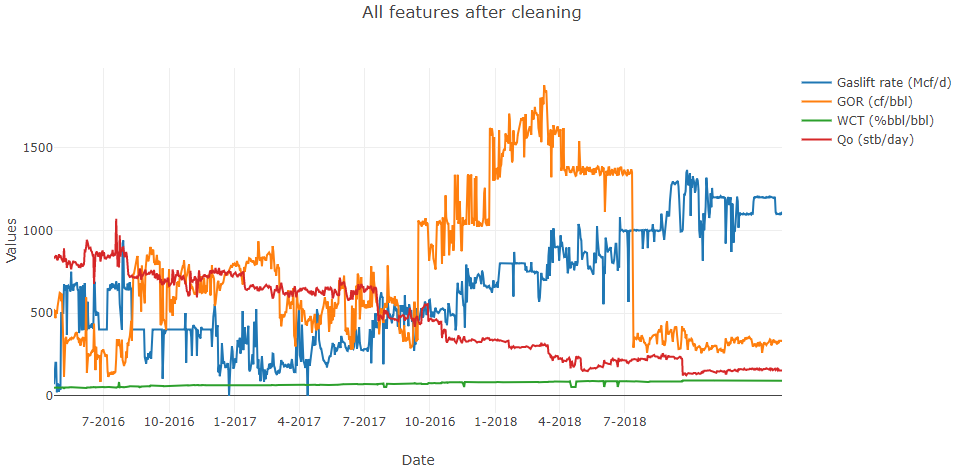
\includegraphics[scale=0.55]{fig/after.PNG}
        \caption{Bộ dữ liệu sau khi được làm sạch}
        \label{fig:after}
    \end{figure}
\clearpage
\subsection{Chuyển vị dữ liệu}
Đối với các dạng dữ liệu theo thời gian, bộ dữ liệu cần được đưa thêm một thuộc tính mới là thuộc tính đầu ra chuyển vị n bước (với n là thời gian dự báo) với mô hình này $n = 1$.\\
Bộ dữ liệu mới như sau:
    \begin{table}[h]
    \centering
    \caption{Năm hàng đầu của bộ dữ liệu mới}
    \begin{tabular}{@{}ccccc@{}}
    \toprule
    \textbf{\begin{tabular}[c]{@{}c@{}}Qgl\\ Mcf/d\end{tabular}} & \textbf{\begin{tabular}[c]{@{}c@{}}GOR\\ cf/bbl\end{tabular}} & \textbf{\begin{tabular}[c]{@{}c@{}}WCT\\ \%bbl/bbl\end{tabular}} & \textbf{\begin{tabular}[c]{@{}c@{}}new\\ STB/d\end{tabular}} & \textbf{\begin{tabular}[c]{@{}c@{}}Qo\\ STB/d\end{tabular}} \\ \midrule
    70.0                                                         & 525.0                                                         & 49.09                                                            & 843.59                                                       & 836.69                                                      \\
    150.0                                                        & 477.0                                                         & 49.77                                                            & 836.69                                                       & 842.81                                                      \\
    200.0                                                        & 469.0                                                         & 49.66                                                            & 842.81                                                       & 849.36                                                      \\
    200.0                                                        & 515.0                                                         & 48.87                                                            & 849.36                                                       & 827.09                                                      \\
    54.0                                                         & 495.0                                                         & 49.93                                                            & 827.09                                                       & 819.58                                                      \\ \bottomrule
    \end{tabular}
    \end{table}
\newline
Với 1019 điểm dữ liệu bắt đầu từ ngày 4/23/2016.
\section{Cấu trúc mạng MLP}
Mô hình được xác lập với một lớp đầu vào có 5 nút, một lớp đầu ra có 1 nút và không có lớp ẩn.
\newline
\def\layersep{2.5cm}
\begin{tikzpicture}[shorten >=1pt,->,draw=black!50, node distance=\layersep]
    \tikzstyle{every pin edge}=[<-,shorten <=1pt]
    \tikzstyle{neuron}=[circle,fill=black!25,minimum size=17pt,inner sep=0pt]
    \tikzstyle{input neuron}=[neuron, fill=green!50];
    \tikzstyle{output neuron}=[neuron, fill=red!50];
    \tikzstyle{hidden neuron}=[neuron, fill=blue!50];
    \tikzstyle{annot} = [text width=4em, text centered]

    % Draw the input layer nodes
    \foreach \name / \y in {1,...,5}
    % This is the same as writing \foreach \name / \y in {1/1,2/2,3/3,4/4}
        \node[input neuron, pin=left:Input \#\y] (I-\name) at (1,-\y + 0.5) {};

    \node[output neuron,pin={[pin edge={->}]right:Output}, right of=I-3] (O) {};

    \foreach \source in {1,...,5}
        \path (I-\source) edge (O);

    % Annotate the layers
    \node[annot] at (1, 0.5) {Input Layer};
    \node[annot] at (3.5, 0.5) {Output Layer};
\end{tikzpicture}
\newline

\subsection{Huấn luyện mô hình}
Mô hình được huấn luyện và cho kết quả như sau:
\newpage
    \begin{figure}[h]
        \centering
        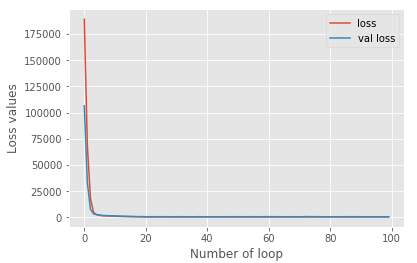
\includegraphics[scale=1.3]{fig/loss.png}
        \caption{Mất mát của hàm tối ưu sau 100 vòng lặp}
        \label{fig:loss}
    \end{figure}
Giá trị mất mát rất thấp, hội tụ sau khoảng 20 vòng lặp.
\clearpage
\section{Dự đoán và đánh giá kết quả}
\subsection{Dự đoán}
Kết quả dự đoán theo thời gian được thể hiện trên đồ thị Hình \ref{fig:evalua} cho thấy kết quả rất khả quan.
    \begin{figure}[h]
        \centering
        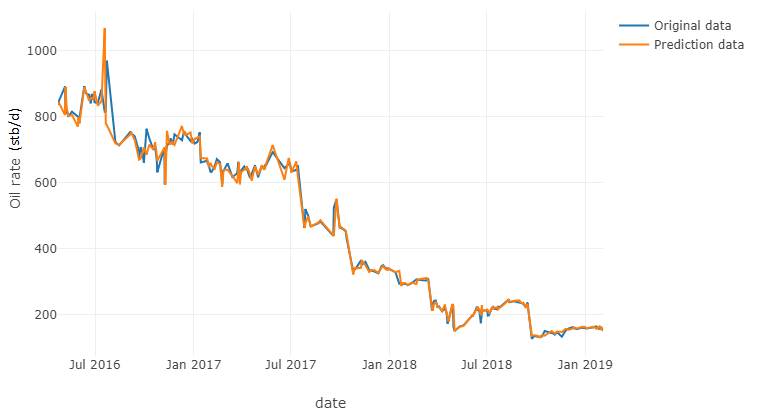
\includegraphics[scale=.85]{fig/evalua.PNG}
        \caption{Kết quả dự đoán}
        \label{fig:evalua}
    \end{figure}
\subsection{Đánh giá}
Kết quả đánh giá được thể hiện như trên Hình \ref{fig:relationship} với $RMSE = 29.62, R^2 = 98.55\%$
    \begin{figure}[h]
        \centering
        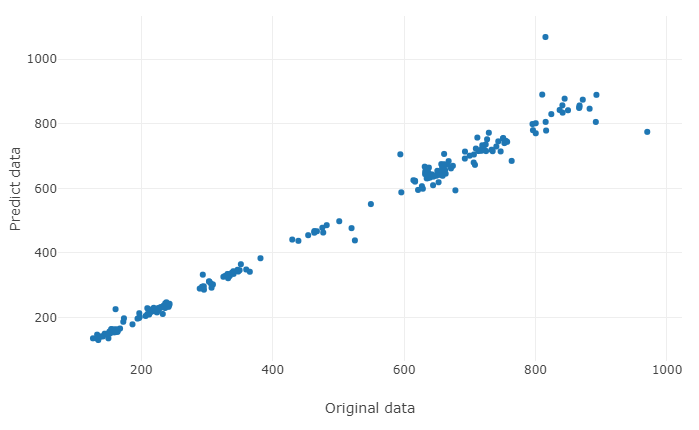
\includegraphics[scale=.85]{fig/relationship.PNG}
        \caption{Đánh giá kết quả}
        \label{fig:relationship}
    \end{figure}


\chapter{NHẬN XÉT ĐÁNH GIÁ VỀ QUÁ TRÌNH THỰC TẬP}
\section{Tự nhận xét về bản thân}
\subsection{Khả năng đáp ứng về kiến thức chuyên môn}
Sau quá trình thực tập tại JVPC, bản thân em nhận thấy rằng các kiến thức chuyên môn và các kĩ năng học tập nghiên cứu thu được từ nhà trường cơ bản đã đáp ứng được các yêu cầu trong các nhiệm vụ được giao tại nơi thực tập.\\
Tuy nhiên, qua quá trình học tập nghiên cứu tại công ty, em nhận thấy các kiến thức thu được từ nhà trường trong bộ môn Công nghệ mỏ vẫn còn đang ở mức cơ bản, khả năng đi sâu vào giải quyết nhiều vấn đề khác nhau vẫn chưa được tốt. Các kĩ năng phân tích, đọc hiểu, xử lý các kết quả đạt được từ phần mềm mô phỏng mới chỉ đáp ứng được yêu cầu cơ bản của công ty.
\subsection{Khả năng đáp ứng về kĩ năng}
Đáp ứng tốt các kĩ năng như làm việc nhóm, làm việc có kế hoạch, làm việc dưới áp lực tiến độ so với yêu cầu của công ty. Đồng thời chấp hành tốt các yêu cầu làm việc và an toàn, các yêu cầu về tinh thần, thái độ làm việc nghiêm túc đã được em chấp hành tốt. Tuy nhiên, trong quá trình thực tập em nhận thấy bản thân còn khá thiếu tự tin trong giao tiếp bằng tiếng Anh đối với các Anh, Chị nước ngoài làm tại công ty, do đó, chưa thể học hỏi được nhiều hơn từ các Anh, Chị trong thời gian này.
\subsection{Các kĩ năng khác}
Các kĩ năng nghiên cứu, tìm hiểu thông tin từ bên ngoài và các kĩ năng nhỏ bên lề đã được em vận dụng tốt.
\section{Nhận xét về Phòng Công nghệ mỏ}
\subsection{Nội dung và công việc được giao}
Phần công việc được giao là vừa sức với sinh viên, mặc dù thời gian còn hạn chế nhưng phù hợp với tình hình thực tế tại công ty.\\
Sinh viên hoàn toàn chủ động trong phần nội dung công việc được giao.
\subsection{Các hướng dẫn của Phòng}
Đơn vị đã giới thiệu cho sinh viên các Anh, Chị hướng dẫn chuyên biệt cho từng phần công việc được giao. Các Anh, Chị hướng dẫn có kiến thức thực tế phong phú, nhiều năm kinh nghiệm trong nghề, đồng thời săn sàng giải đáp nhiều thắc mắc bên lề của sinh viên. Những vấn đề khó khăn hay thắc mắc trong vấn đề học tập sau thực tập được các Anh, Chị tạo điều kiện liên hệ trực tiếp để giải đáp rõ ràng hơn.\\
Ngoài ra, sinh viên còn nhận được sự giúp đỡ từ các Anh, Chị khác trong Phòng.
\subsection{Về quan hệ với các Anh, Chị kỹ sư trong Phòng}
Quan hệ hòa đồng, vui vẻ và cởi mở đồng thời sẵn sàng giải đáp mọi thắc mắc liên quan đến quá trình thực tập với sinh viên.
\section{Nhận xét về cách tổ chức thực tập của Bộ môn}
\subsection{Quy trình, cách thức tổ chức thực tập}
Quy trình và cách thức tổ chức thực tập của Bộ môn nhanh gọn, rõ ràng.
\subsection{Về thời gian và thời điểm tổ chức}
Thời điểm tổ chức thực tập hợp lý (ngay sau khi thi học kì). Thời gian thực tập vừa đủ, hợp lý để sinh viên có thể hoàn thành nhiệm vụ đã đề ra.
\subsection{Về sự chuẩn bị tại Bộ môn}
Bộ môn có sự chuẩn bị tốt cho quá trình thực tập của sinh viên, việc thông báo, nhắc nhở và quản lý sinh viên trong quá trình thực tập luôn được thực hiện thường xuyên.
\newpage
\subsection{Về kiến thức và kĩ năng sinh viên được trang bị}
Kiến thức lý thuyết sinh viên được trang bị cơ bản đã đáp ứng được nhu cầu của quá trình thực tập.\\
Kiến thức thực tế còn nhiều thiếu xót, các kĩ năng phần mềm không được đề cập nhiều trong chương trình học.\\
Kĩ năng phân tích kết quả mô phỏng chưa được đầy đủ.

\chapter{KẾT LUẬN VÀ KIẾN NGHỊ}
\section{Kết luận}
Trong thời gian thực tập tại Công ty Dầu khí Việt-Nhật, về cơ bản em đã hoàn thành được nhiệm vụ đã đề ra:
	\begin{itemize}
    	\item[-] Xây dựng mô hình dự báo khai thác.
    \end{itemize}
\section{Kiến nghị}
Qua quá trình thực tập em nhận thấy kiến thức được học tại Trường còn rất giới hạn, mong rằng các Thầy, Cô bộ môn sẽ sắp xếp để có thể truyền đạt thêm nhiều kiến thức hơn nữa cho sinh viên trong quãng thời gian sắp tới.

\end{document}
